\chapter{Threat model}
\label{model}
In this chapter, we deepen several security weaknesses that affect the current version of LoRaWAN, focusing on privacy-related issues and their implications. 
\\
First, we introduce security policies adopted in designing IoT applications. Next, we investigate information leakages deriving from wireless communications. Finally, we deeply analyze LoRaWAN and model the threats derivated from privacy problems still unresolved.

\section{Security requirements}
Generally, IoT applications are conceived following these security policies \cite{securing_iot}:
\begin{enumerate}
	\item Confidentiality: protecting the data by preventing unauthorized users from accessing private information
	\item Integrity: preventing unauthorized users from modifying the data.
	\item Availability: ensuring that the resources and information are available when requested by authorized users.
	\item Authenticity: ensuring that the transferred data is genuine by authenticating the parties involved in the transmission.
\end{enumerate}
LoRaWAN complies with these principles. It makes use of standard, well-vetted algorithms, and end-to-end security \cite{Moraes2021ASR}. Devices use AES-CTR to encrypt each payload, avoid packet replay carrying a frame counter, and implement Message Integrity Code (MIC). Moreover, as part of the network join procedure, end devices and the LoRaWAN network establish mutual authentication, ensuring only authorized devices can join.

\section{Privacy issues in LPWANs}
In this section, we examine the privacy of LPWANs, and, in particular, of LoRa. As shown in \ref{fig:passive}, since the long communication range of LPWAN technologies allows messages to be received several kilometers away, an eavesdropper, though located many hundred meters from endpoints, can infer sensitive information and fingerprinting devices.
\begin{figure}[ht]
    \centering
    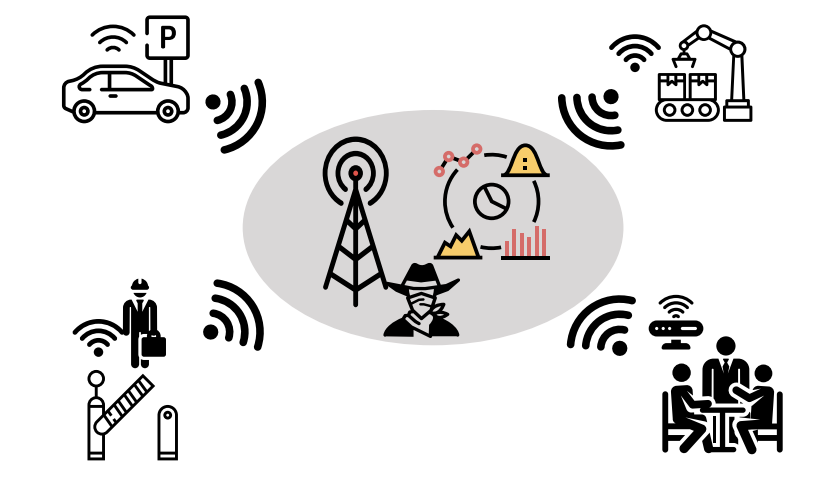
\includegraphics[width=0.7\linewidth]{images/threat/passive_adversary.png}
    \caption{When end devices transmit messages to the Application Server, the passive adversary is able to deduce sensitive information.}
    \label{fig:passive}
\end{figure}
In detail, we assume that the passive adversary is equipped with one or more receivers collecting end device transmissions, it is within the communication range of at least one gateway, and that it has a \textit{priori} knowledge about the application associated with an ED.

\subsubsection{Fingerprinting}
LoRa devices can be uniquely recognized using physical (PHY) layer fingerprinting \cite{inproceedings},  a technique that leverages based on small differences in the analog RF signals sent by wireless devices, caused by imperfections introduced in the analog hardware components during the manufacturing process \cite{10.1145/1409944.1409959}.

\subsubsection{Information leakages}
Unlike other protocols, LPWAN is technology-constrained, making it easier for attackers to reconstruct a view on the network they monitor. While other wireless devices transmit messages not necessarily related to real situations, LPWAN sensors are simpler and often dedicated to no more than one function, such as the transition of data when an event occurs. Moreover, the LPWAN event space is small and binary, making the purpose of the individual sensors clearer. Just consider the case of a parking system application that notifies clients if a given parking lot is occupied or not \cite{app10134674}. LoRa endpoints simply send binary messages (the lot is empty, the lot is not empty) only when there is a change of state (a vehicle left the lot). In absence of obfuscation techniques, a potential attacker recognizes the presence of real messages by simply eavesdropping on the LPWAN channel. Not only: a deviation from standard transmission behavior also presupposes the occurrence of an event. For example, in the case of an application that monitors the availability of a meeting room, the LoRa sensor transmits less when there is a series of long meetings that keep the room busy. The eavesdropper, collecting the messages in a given time frame, can perform traffic analysis to extrapolate the transmission behavior and gain information about given circumstances. 

\section{Re-Identifying addresses in LoRaWAN}
\label{address_identification}
In this works, we focus on a privacy threat correlated to two LoRaWAN addresses: the DevAddr and the DevEUI. LoRaWAN avoids exposing to eavesdroppers sensitive information concerning devices and the network they are. For a given endpoint, only the application and the network knew the association between the current DevAddress and the DevEUI. Since DevEUI is revealed only during the OTAA procedure and the DevAddress is sent only in uplink messages, an ED can't send a packet with both identifiers exposed.
\\
The decoupling of the DevEUI from the DevAddress guarantees devices' anonymity. In detail, the NwkID field contained in the DevAddress reveals information about the network, and the OUI field of DevEUI contains information about the constructor of the device. And, by combining these two elements, the attacker increases its knowledge about the targeted LoRaWAN network. For example, it can determine which devices from a given operator (OUI) are around an assigned gateway (NwkID) or if the network belongs to private or experimental projects. Several studies demonstrate that the current LoRaWAN specification is not strong enough to assure that the association of these addresses remains unknown to unauthorized parts. A technique proposed in \cite{tech2020} recognizes the DevAddress-DevEUI association relying on the timing between a Join-Request and the immediately following uplink message. On the opposite, this research \cite{devil} goes further: it underlines that this temporal linking is not always constant and proposes a pattern-based approach, named DEVIL, which, tested on a real dataset provided by an Italian operator, declares more accurate results. DEVIL is a batch-type algorithm: it processes all the data a posteriori, collecting uplink and join request messages in a given time window and elaborating them later. In this work, we exploit the advantages of pattern matching and develop a real-time defensive strategy that can prevent attacks such as those mentioned above.